\chapter{Learning motion primitives for manipulation tasks}
\label{cha5}

\section{Introduction}
\label{cha5:sec1}
The focus of this chapter is learning reaching motion for manipulation. In previous chapters, we discuss learning multi-finger grasping and adaptive control strategy. These are done at the ``end effector level'' and rely on the robot limb to deliver the end effector to a proper position. In this chapter, we study how to program a robot to reach a target object with a trajectory satisfying the task constraints. This is achieved by, again, the program by demonstration technique where human demonstrate the primitive reaching motions. The robot then execute the motions and find out the boundary of the motions with its embodiment. 
In addition to learning, we label the motions with human language so that the robot will be able to ``understand'' the motion and react to human commands referring to the labels. 

\paragraph{Motion primitive} ~\\
To accomplish a more complex task, a sequence of motions is needed. As discussed in the introduction chapter, the high dimensional search space makes this sequence of motion difficult to generate. To reduce the search space, the concept of motion primitives in neuroscience~\citep{bizzi2008combining} has been introduced to planning. The basic principle is to discretize a manipulation task into a set of motion primitives, with each serving an elementary manipulation function. After modelling each primitive, the whole task then can be achieved by coordinating them properly.

Modelling motion primitives remains an open problem. Much literature discusses how to design motion primitives that accomplish specific tasks ~\citep{michelman1994forming,felip2012manipulation,ijspeert2013dynamical}. In those works motion primitives are modelled as a set of differential equations or control rules. New motions are generated by tuning the parameters in the models. Deriving these equations and control policies is not an easy task, neither is fine tuning the parameters to generate new motions. These activities require a deep understanding of the task and the dynamic model.

These difficulties can be alleviated by using the learning by demonstration approach and modelling the motion in state space. In this chapter we propose an easy to use system for learning manipulation motion primitives from human demonstration. To achieve this goal, we exploit the application of the mimesis model~\citep{inamura2004embodied} in learning motion primitives for object manipulation.

\begin{figure}
  \centering
  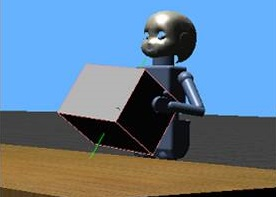
\includegraphics[width=6cm]{./fig_cha5/begin.jpg}
  \caption{ \scriptsize{iCub grasping a box with both arms}
}
    \label{begin}
    \vspace{-0.5cm}
\end{figure}



\paragraph{Mirror neurons and Mimesis Model} ~\\
The mimesis model is a mathematical realization of the function of the mirror neurons. Mirror neurons are a kind of neuron found in primates and birds, which fires both when the animals observe and execute a motion. In the human brain, mirror neurons has been identified
in the area of the premotor cortex, the supplementary motor area, the primary somatosensory cortex and the inferior parietal cortex. These areas contribute to human control of motion and sensory reception. It is generally believed that mirror neurons are associated with an animal's ability to learn by imitation and to understand the action of others~\citep{rizzolatti2004mirror}. Motivated by this idea, many researchers try to understand the function of mirror neurons and hence implement it on robots to equip them with human level imitation and learning ability. We are also inspired by this idea and hence try to mimic the mechanism of mirror neurons to learn manipulation motion primitives.

The mimesis model is developed to realize the functions of the mirror neurons: observe motion, recognize motion and generate motion.
This mimesis model has been shown to be effective in motion recognition, generation and robot coaching~\citep{inamura2008geometric,okuno2011motion}. It is built based on the Hidden Markov Model (HMM).
In the mimesis model, all demonstrated motion patterns are first encoded by a HMM. These HMMs are then projected to a topological space called ``proto-symbol space''. In this space, each HMM is projected as a point called a ``proto-symbol'', and is labelled by the character of its representing motion, such as ``grasp low box" or ``grasp high box". The similarity between two motions (HMMs) is represented as the Euclidean distance between their proto-symbol.

Recognition of an unknown motion is achieved by projecting the unknown motion to the proto-symbol space. This gives us a new proto-symbol. If the new proto-symbol is very close to a known proto-symbol, then it is very likely the unknown motion is the motion represented by the closest proto-symbol. On the other hand, new motion generation is achieved by exploring new proto-symbols, i.e. interpolating between the known proto-symbols. The new motions generated will be similar to, but different from, the motions encoded by the surrounding proto-symbols.

As we label each proto-symbol, the mimesis model provides a base of understanding of human and robot behaviour. This even allows the robot user to adjust robot motion using natural language. For example, starting from the ``gasp low box" motion, we can instruct the robot to raise its arms higher to grasp a box on the top of a cabinet using the command ``not high enough, go higher to grasp". This command will generate a motion closer to the motion labelled by ``grasp high box".

Most of previous work of the mimesis model focuses on learning whole body movements. Our work extends the mimesis model to learn motions of manipulation that involve interaction with objects.
The work of Kunori et al.~\citep{kunori2009associating} using hidden Markov models to encode motion primitives for object manipulation has a similar concept to our work. While they focused on extracting key features and reshaping movements for good performance, we focus on combining known manipulation motion primitives to generate new motions that can achieve the desired effects. Although interpolation of known motions is not new in motion synthesis~\citep{hoshino2004interpolation,glardon2004pca}, most of the existing work focuses on free body motion. The application to object manipulation is rarely discussed.

The goal of this work is to develop an easy to use system for the robot to learn manipulation motion primitives and generate new motions to adapt to unseen scenarios. The system is implemented for a bi-manual grasping task. Different to the static fingertip grasping synthesis~\ref{cha3}, in this task we focus on the grasp reaching motion.

\section{Learning by mimesis model}
\label{cha5:sec2}

We adopt the mimesis model to learn motion primitives of manipulation from human demonstrations. In this approach, the demonstrated motions are firstly encoded by the Hidden Markov Model (HMM)~\citep{rabiner1989tutorial}. A topological space, i.e. proto symbol space, is then constructed to represent the similarities between the HMMs. In this space, each HMM is abstracted to a labelled point: the proto symbol. New motions are generated as new proto symbols. The correlation between the location of the new proto symbols and their physical effects is learnt by regression. This correlation allows us to directly query a new motion from a high level task requirement.

In short, the general approach has 5 steps as listed underneath:

\begin{enumerate}
\item {\bf{Human demonstration of motion primitives}}: A human teacher demonstrates manipulation motion primitives (Section~\ref{cha5:sec2:demonstration}).
\item {\bf{Motion symbolization}}: Abstract the motion primitives by HMM and create the proto-symbol space (Section~\ref{cha5:sec2:symbolization}).
\item {\bf{Motion interpolation}}: Interpolate the proto-symbol space and construct new HMM.  (Section~\ref{cha5:sec2:interpolation}).
\item {\bf{New motion generation}}: Generate motion using proto-symbols (Section~\ref{cha5:sec2:generating}).
\item {\bf{Learning motion effects}}: Robot reproduces the motion and learns the correlation between the location of the proto-symbols and the effect of the generated motions (Section~\ref{cha5:sec2:learning}).
%\item {\bf{Generating}}: Given a unseen object, choose a proper point in the proto-symbol space and generate the corresponding motion sequence to grasp the object (Section 3E).
\end{enumerate}



\subsection{Human demonstration of motion primitives}
\label{cha5:sec2:demonstration}
%To design a adaptive motion primitive, demonstrations showing different scenarios are required.
The motion primitives of manipulation are first demonstrated by a human. The same primitives were demonstrated a few times so that the HMM is able to encode the general features of the movement. Each primitive has its own purpose and distinct pattern. To enable the robot to work in different task contexts, different primitives need to be demonstrated. For example, to design a motion primitive for fetching boxes in different sizes (size is the task context), we need to demonstrate at least two primitives: grasping a small box and grasping a big box (Figure.~\ref{fig:bimanual}). Grasping a box with the size between the big one and the small one is achieved by interpolation between these primitives. For more complex motion, more than two primitives may be required to achieve the desired motions.

%Later in the interpolation step (section~\ref{sbsec:interpolation}), new motions are generated by combining the demonstrated motions.
In this approach, the demonstrated motions do not only provide the dynamics of the motion primitives, but also define the feasibilities of the motion primitives. In the example given above of grasping different sizes of boxes, one should demonstrate the motion primitive for grasping the smallest feasible box and the other for grasping the biggest feasible box. Here the ``feasibility'' is defined according to the limitation of the robot joints. As the new motions are interpolations of the demonstrations, joint limits or singularities can be avoided in the new motions by well chosen demonstrations.

\begin{figure}
\centering
  \subfloat[\scriptsize{}]{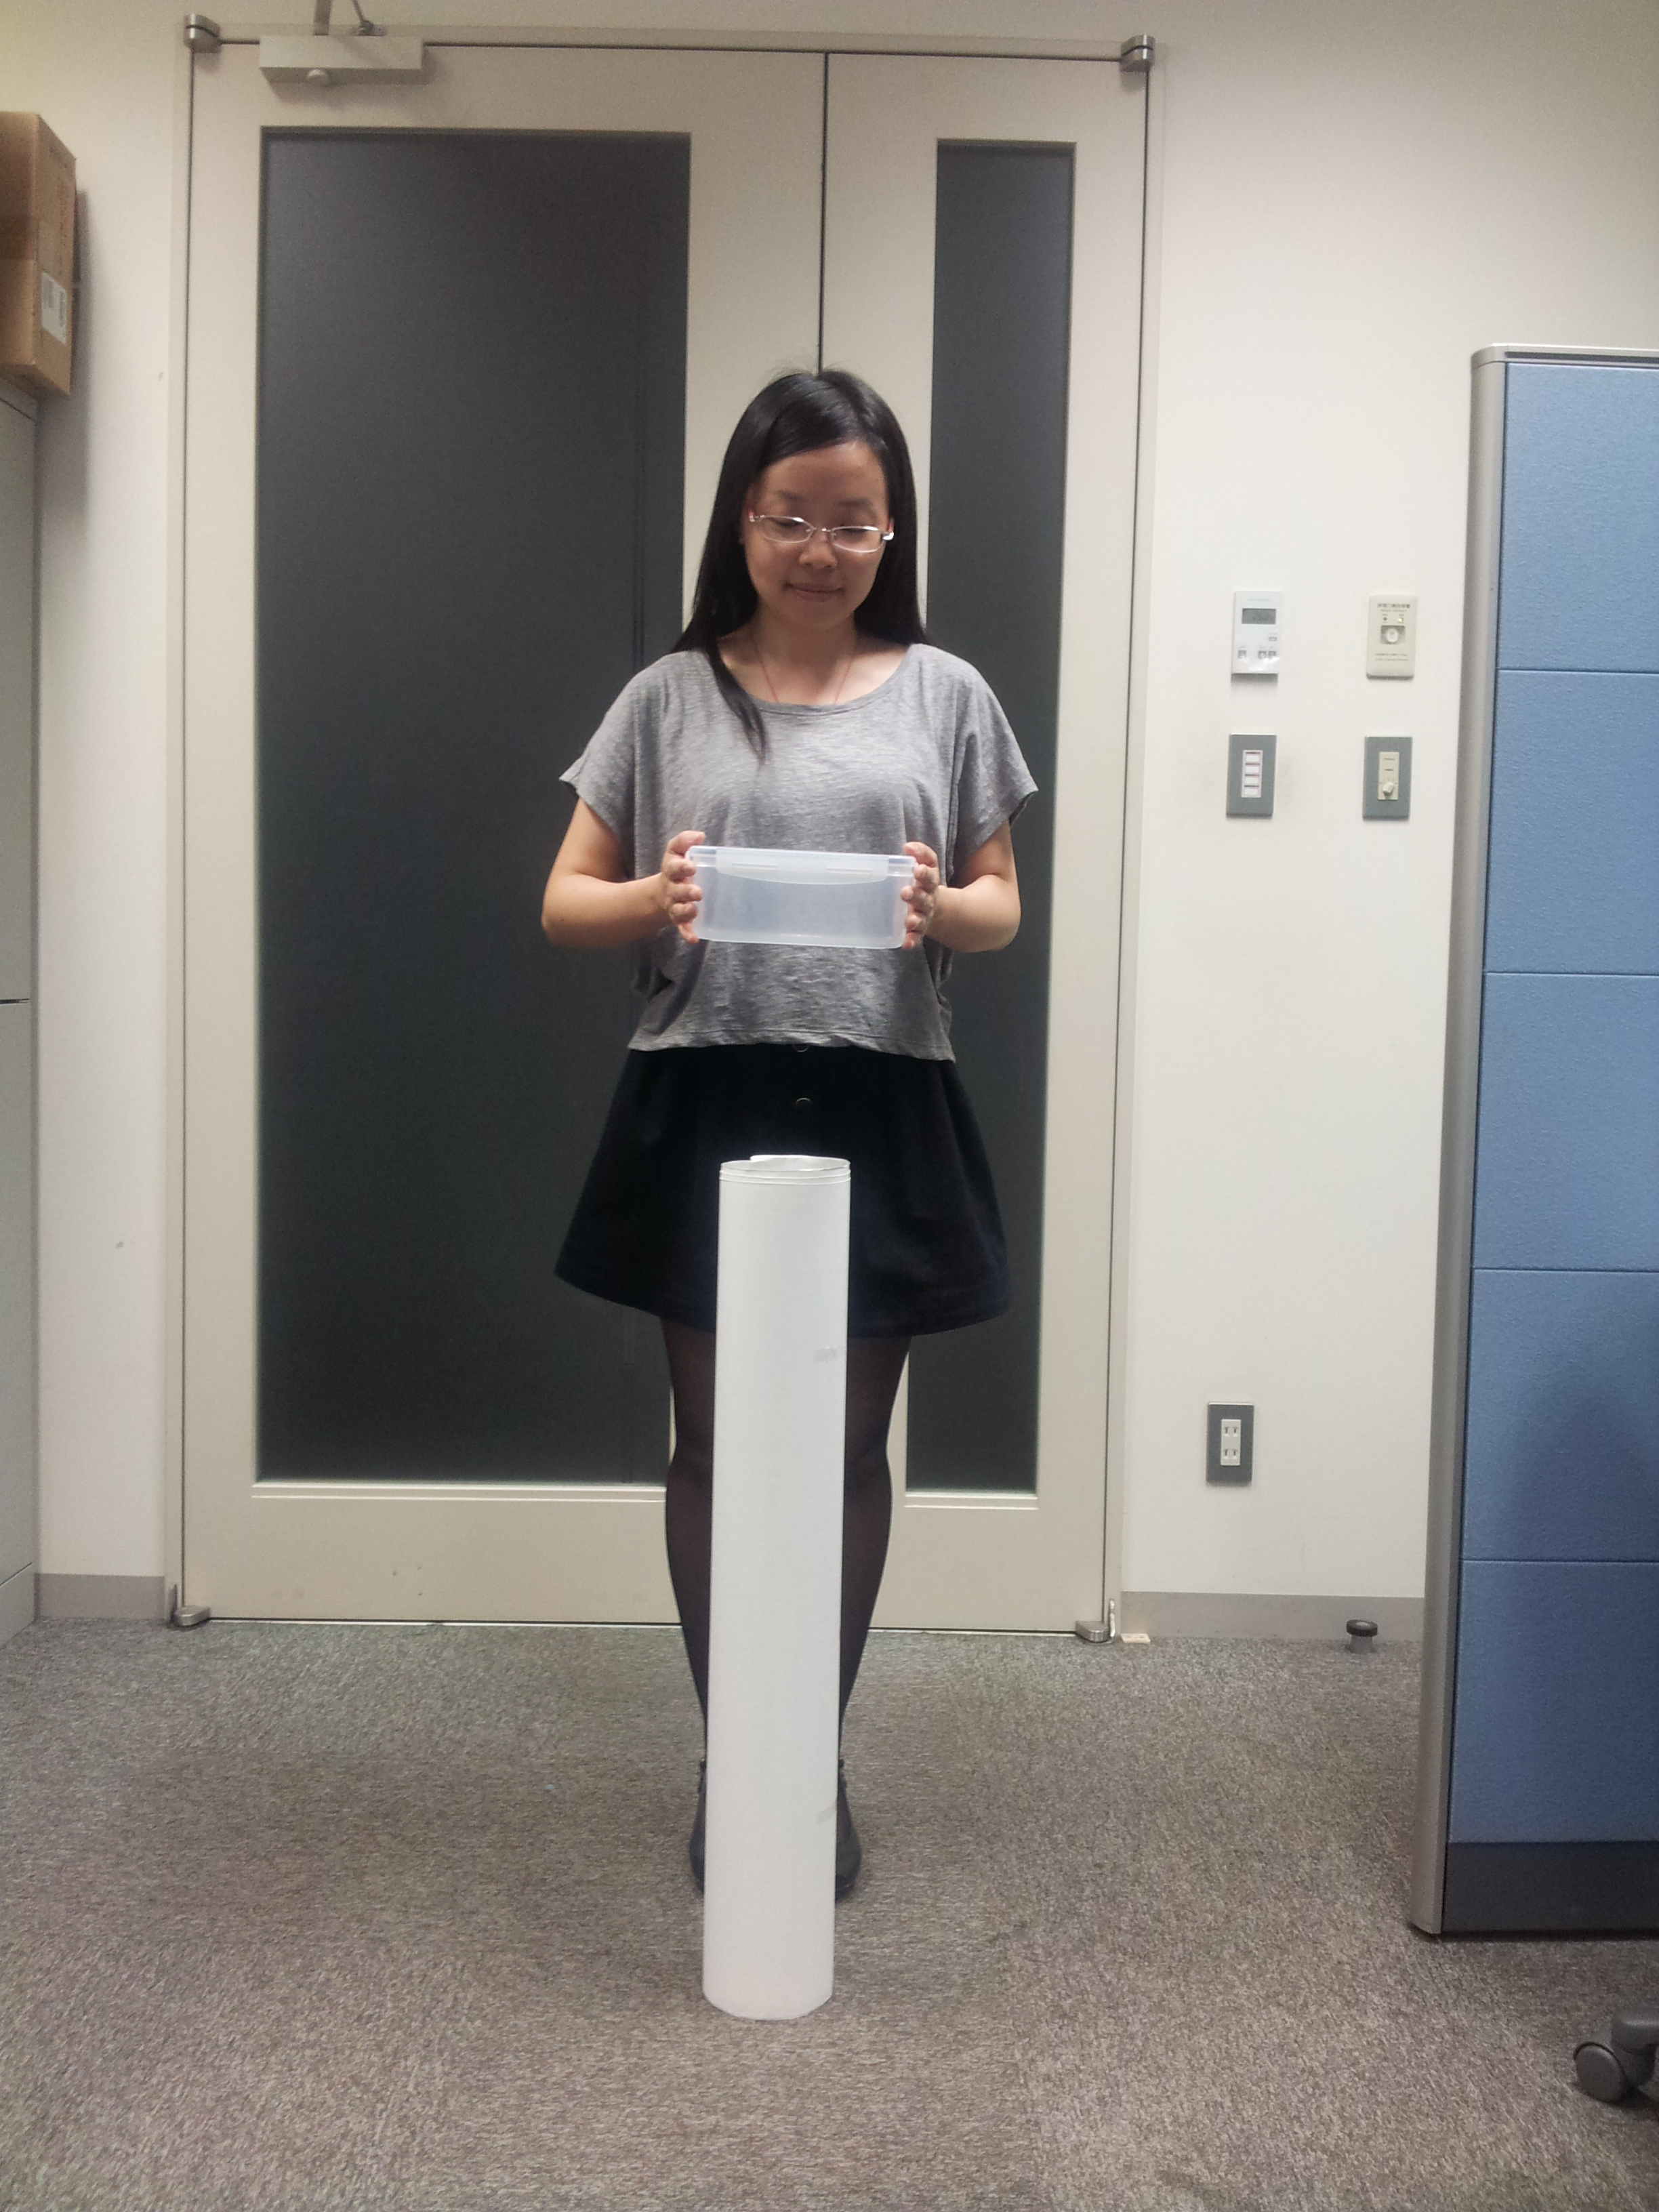
\includegraphics[width=5cm]{./fig_cha5/gsbox.jpg}}
  \subfloat[\scriptsize{}]{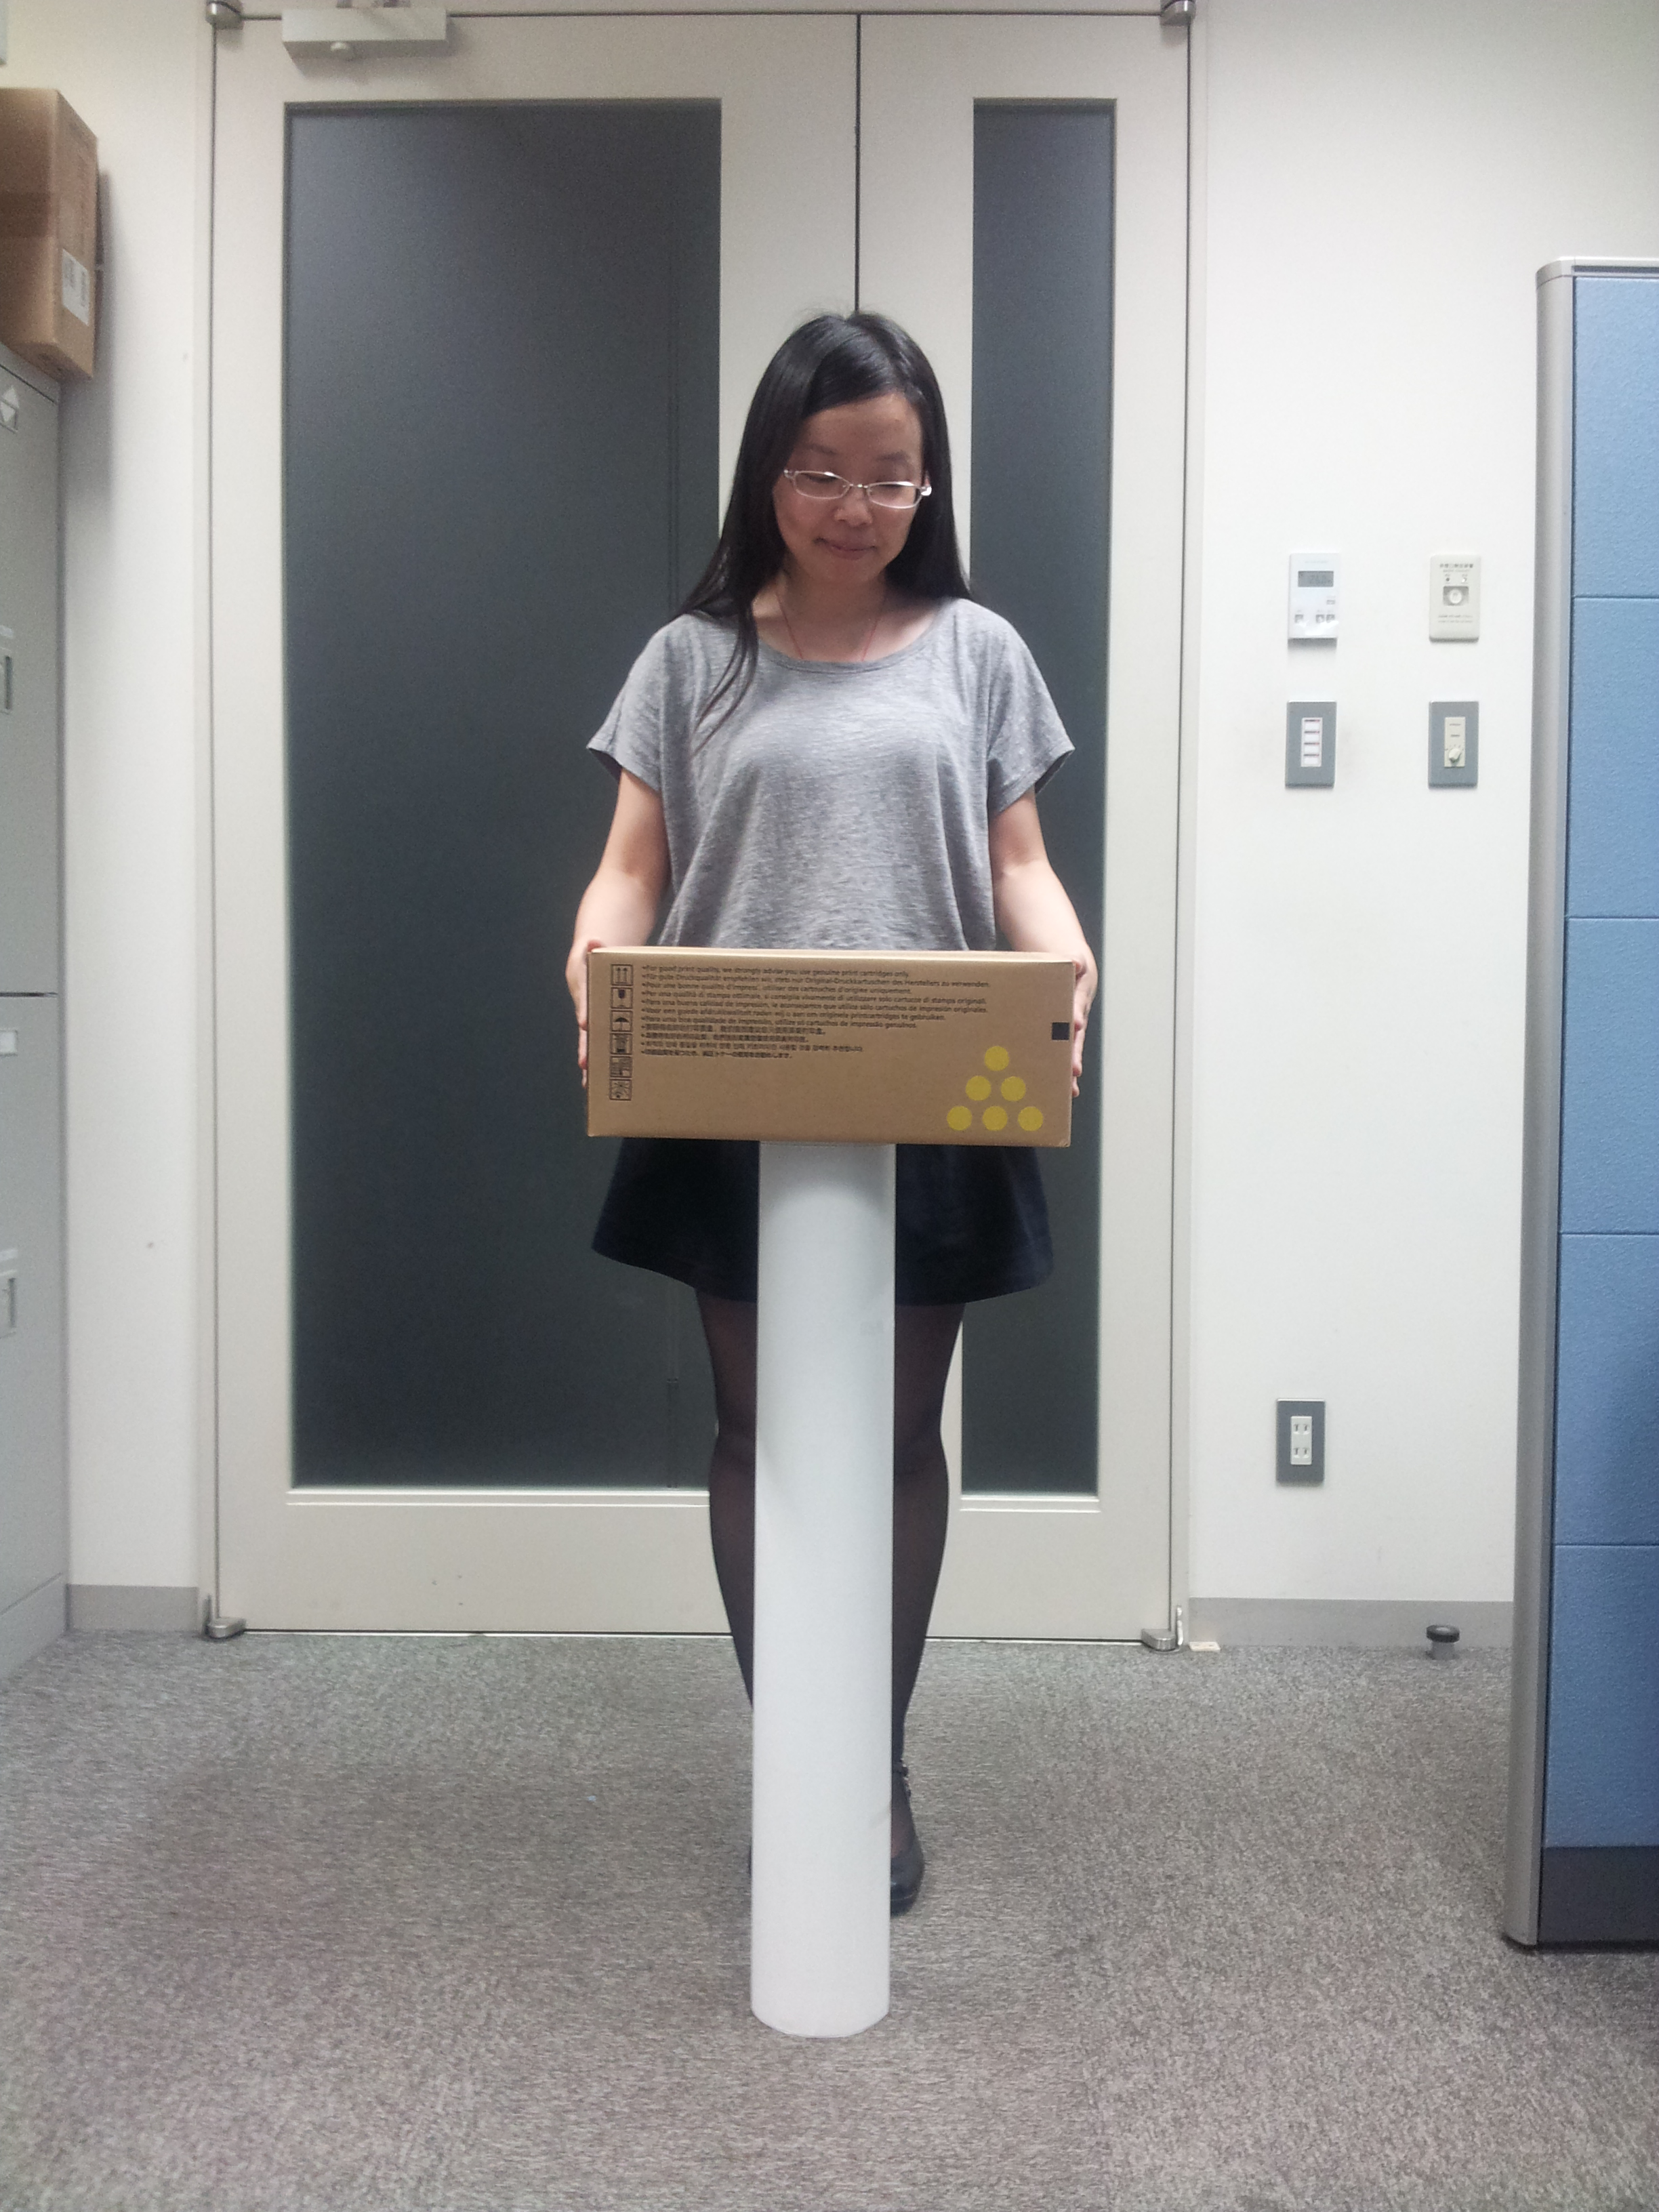
\includegraphics[width=5cm]{./fig_cha5/gpinkbox.jpg}}
  \caption{ \scriptsize{Human bimanual grasps. (a) Human grasping a small box. (b) Human grasping a big box.}}
  \label{fig:bimanual}
\end{figure}


\subsection{Motion symbolization}
\label{cha5:sec2:symbolization}
%The demonstrated motion sequences are then adapted to a 20 degrees of freedom humanoid, the HOAP robot~\citep{inamura2004embodied}.
In order to store and label the observed motions, we construct the ``proto-symbol space''. This is done in two steps: first encode the motion patterns as HMM's, and second project them to be a set of ``proto-symbols'' in the proto-symbol space, where the similarity between different motion patterns are represented by the Euclidean distance.

\paragraph{Hidden Markov Model} ~\\
%TODO: more HMM
%TODO: more forward-backward procedure
A Hidden Markov Model is a stochastic mathematical model for sequential data. It describes a data sequence as a Markov process, with which the data is described by transitions between a set of states. In a Markov process, the future state of the process depends solely on its current state. It can be thought of as a 'memory-less' process: it only need to 'remember' the current state but not the whole process' history, in order to predict the future. This is a strong assumption.
Temporal patterns with this characteristic, e.g. speech, handwriting and sequences of body movements, can be approximated by a Markov model. In a simple Markov process, the transitions between states are directly visible. Conversely, the states of hidden Markov Model is not directly visible, i.e. hidden.

An HMM has two layers: the hidden states and the outputs. The outputs are directly visible but their pattern is controlled by the hidden states. The way the hidden states transit to each other and the way they emit to the outputs determine the output pattern. Though they are not directly visible, the hidden states can be inferred by the observable outputs. A well known application of HMM is speech recognition. Speech recognition systems use HMM to analyze the signal of speech in order to discover the meaning. Here the sound of the speech is the observable output and the meaning of the speech is the hidden state.


A HMM can be fully described by a triple $\left(\pi,\boldsymbol{A},\boldsymbol{B}\right)$:

\begin{enumerate}
\item $\pi$: the vector of the initial probabilities of each state.
\item $\boldsymbol{A}={a_{ij}}$: the state transition matrix. This is the probability that one state ($q_i$) transits to another ($q_j$): $Pr\left(q_i{\mid}q_j\right)$.
\item $\boldsymbol{B}={b_{ij}}$: the output probability (confusion matrix). This is the probability that one state ($q_j$) produces an output ($o_i$): $Pr\left(o_i{\mid}q_{j}\right)$. If the outputs are discrete, i.e. have a countable number of states, this can be simply represented by a matrix. If the outputs are continuous, the output probability is usually described by a GMM.
\end{enumerate}

Figure~\ref{fig:chmm} illustrates the mechanism of a HMM encoding a motion pattern. This is a left-to-right Continuous Hidden Markov Model (CHMM). In a general HMM, the hidden states can transition to any other states. In a left-to-right HMM the transition has more constraints. The states are placed in a ``left to right'' order, each state can only transition to the state at its right or transition to back to itself, the possibility of it transiting to any other states is zero. A left-to-right HMM restricts the complexity of the data pattern it can model and is adequate for modelling motion primitives.

To encode the motion primitives by HMM, we define the pattern by: $\lambda$ = $\{\boldsymbol{Q},\pi,\boldsymbol{A},\boldsymbol{B}\}$, where $\boldsymbol{Q}=\{q_1, ..., q_N\}$ is a finite set of states, $\pi$ is the the initial distribution, $\boldsymbol{A}=\{a_{ij}\}$ is the state transition probability matrix denoting the probability that node $q_i$ transits to $q_j$ and $\boldsymbol{B}=\{b_{i}\}$ is the continuous output probabilities denoting the probability distribution that the output vector $o[t]$ is given by $q_i$. The $\pi$ is the same as for each CHMM as we use a left-to-right CHMM model. Therefore, the parameter set $\mathcal{P} = \{a_{ij},b_i\}$ characterizes the behaviour of the motion primitive. We call $\mathcal{P}$ a proto-symbol.

The CHMM is learned using the Baum-Welch algorithm~\citep{rabiner1989tutorial}\footnote{We use the Hidden Markov Model Toolkit (HTK) to learn the HMM}.
For simplicity, we use a single Gaussian model for the output of each node in the CHMM. This allows us to synthesise new motion simply by interpolating the means and covariances of the Gaussians (Section~\ref{cha5:sec2:interpolation}).

The proto-symbol space is constructed to represent the similarity between CHMMs. This requires us to compute the similarity between each pair of CHMMs. In this work, we use the Bhattacharyya distance~\citep{kailath1967divergence} as our similarity metric, as it is a symmetric metric with respect to two probability variables. The Bhattacharyya distance $BD(p,q)$ between two Gaussian distributions $p(x;\mu_p,\Sigma_p)$ and $q(x;\mu_q,\Sigma_q)$ is defined as follows:


\begin{figure}[t!]
  \centering
  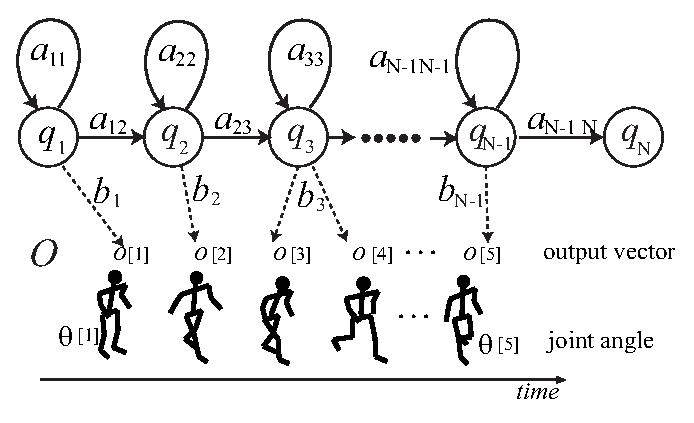
\includegraphics[width=14cm]{./fig_cha5/chmm.eps}
  \caption{ \scriptsize{An illustration of encoding a motion by Continuous Hidden Markov Model\protect\footnotemark.}
}
    \label{fig:chmm}
\end{figure}

\footnotetext{Reprinted with permission.}

%\begin{equation}
\begin{align}
\begin{split}
&BD(p,q) = -log\int^{\infty}_{-\infty}\sqrt{p(x)q(x)}dx \\
=\frac{1}{8}&\mu_{pq}\left({\frac{\Sigma_p+\Sigma_q}{2}}\right)^{-1}\mu_{pq}^T +\frac{1}{2}log{\frac{\mid\frac{\Sigma_p+\Sigma_q}{2}\mid}{\mid\Sigma_p\mid^{\frac{1}{2}}\mid \Sigma_q\mid^{\frac{1}{2}}}}
\end{split}
\end{align}
%\end{equation}
where
\begin{equation}
\mu_{pq} = \mu_p - \mu_q
\end{equation}

The Bhattacharyya distance DB($\lambda_1, \lambda_2$) between two HMMs is computed by summing the distances between the Gaussian distributions, i.e. the output probability distributions for the nodes:

\begin{align}
\begin{split}
&DB(\lambda_1, \lambda_2) = \\
&\sum_i\sqrt{BD\left(\mathcal{N}_{1i}\left(\mu_{1i},\Sigma_{1i}\right), \mathcal{N}_{2i}\left(\mu_{2i},\Sigma_{2i}\right)\right)}
\end{split}
\end{align}
where $\mathcal{N}_{ji}(\mu_{ji},\Sigma_{ji})$ is the output probability at the $i$-th node $q_i$ of the HMM $\lambda_i$.

The proto-symbol space is constructed by the multi-dimensional scaling technique (MDS)~\citep{schiffman1981introduction}. This technique computes the locations of the CHMMs in the proto-symbol space by minimizing the criterion:

\begin{equation}
S^2 = \sum_{i,j}\left(DB_{ij}-d_{ij}\right)
\end{equation}
where $DB_{ij}$ is the Bhattacharyya distance between the $i$th and $j$th CHMMs and $d_{ij}$ is their Euclidean distance between their proto-symbols. %Figure~\ref{pss} shows an proto-symbol space constructed by 4 proto-symbols.



\subsection{Motion interpolation}
\label{cha5:sec2:interpolation}
To generate new motions, new locations in the proto-symbol space are explored. This is done by interpolation between different proto-symbols.
%For the same set of motion primitives, the number of states are the same and hence the motions can be mixed in the time domain.
In the left-to-right model, the expected duration $s_i$ of the state $q_i$ can be computed as

\begin{equation}
\label{sequation}
s_i = \sum_{n=1}^{\infty} n(1-a_{ii})a_{ii}^{n-1} = \frac{1}{1-a_{ii}},
\end{equation}
where $a_{ii}$ is the probability of self-transition at the state $q_i$.

A new proto-symbol $\hat{\mathcal{P}}$ is expressed by the linear combination of $m$ proto-symbols $(\mathcal{P}_1, ..., \mathcal{P}_m)$. The weights of different proto-symbols are expressed by the mix coefficient $c_j$. The expected duration $\hat{s}_i$ for the new motion in the state $q_i$ is computed as

\begin{equation}
\hat{s}_i = \sum_j^mc_js_i^{(j)}
\label{s}
\end{equation}
with this we can compute the new state transition probability $\hat{a}_{ii}$ as

\begin{equation}
\hat{a}_{ii} = \frac{\hat{s}_i-1}{\hat{s}_i}
\end{equation}
Note that according to the Eq.~\ref{s}, $s_i\ge1$ and hence the following constraint must be satisfied

\begin{equation}
\sum_j^m\frac{c_j}{1-a^j_{ii}} \ge 1
\end{equation}

To compute the new output probability $b_i$, since there is only one Gaussian in each state, we simply sum the means and variances of the Gaussians of the same state as

\begin{equation}
\hat{b}_i(O) = \mathcal{N}(O;\hat{\boldsymbol{\mu}}_i,\hat{\boldsymbol{\sigma}}_i^2) = \sum_j^m{c_jb_i^{(j)}(O)}
\end{equation}
where
\begin{equation}
\hat{\boldsymbol{\mu}}_i = \sum_j^mc_j\boldsymbol{\mu}_i^{(j)}
\end{equation}

\begin{equation}
\hat{\boldsymbol{\sigma}}_i^2 = \sum_j^mc_j^2{\boldsymbol{\sigma}_i^{(j)}}^2
\end{equation}
$\mu_i^{(j)}$ and ${\sigma_i^{(j)}}$ are the mean and variance of the Gaussian representing the $i$-th state.

In theory this method can also be used to extrapolate the proto-symbols with negative mixing coefficients, which allows us to explore outside the feasible region defined by the demonstrations. This can generate motions that are beyond our experience however the feasibility cannot be guaranteed, i.e. this may gives joint angles over the robot's limit.

\subsection{Motion generation}
\label{cha5:sec2:generating}
A new motion sequence is generated from the new proto-symbols by using an averaging method~\citep{inamura2004embodied}.
%The basic idea is to decode a motion sequence from the CHMMs by averaging over repetition of motion generation.
The steps of generation are as follows :

\begin{enumerate}
\item: Starting from a node $q_1$, let the motion element sequence be $O = \phi$.
\item: Use the transition probability $\{a_{ij}\}$ to generate the states $q_j$.
\item: Use the output probabilities $\{b_i\}$ to decide the output label $o_k$.
\item: Add the output label $o_k$ to the motion elements sequence $O$.
\item: Stop when the generation process reaches the end node $q_N$.
\end{enumerate}

Due to the stochastic nature of this method, motions generated by the same HMM are not identical at each time. Nevertheless, they have the same dynamics as they are generated from the same parameters $\boldsymbol{A}$ and $\boldsymbol{B}$. We repeat the above steps and average the generated motions to produce the final motion. As the duration of each generated motion is different, prior to averaging we match the time in each motion by:

\begin{equation}
\bar{\theta}\left(t\right)=\theta\left(T\frac{t}{T_{adv}}\right)
\end{equation}

where $T$ is the time duration of each motion, and $T_{adv}$ is the average time duration of all motions. This step normalize all motions in the scale of time.

\subsection{Learning motion effects}
\label{cha5:sec2:learning}

In contrast to free body motions, the motion of object manipulation needs to achieve certain outcomes, such as grasping a given size of box. However the physical effects of the demonstrated and generated motions are unknown, as the robot has a different embodiment to the human demonstrator. For example, the motion for a human to grasp a 30$cm$ length box may only allow the robot to grasp a 15$cm$ length box. Therefore, a learning process is needed to quantify the correlation between the location of the new proto-symbol and its physical effect.

To do this, we first interpolate the proto-symbol space with a few different mixing coefficients. We then generate the corresponding motions and perform them with a robot. The platform we used is the iCub in the Webots simulator. As the iCub has the same joint configuration of arm as the one provided by Kinect, we directly apply the generated motions to the iCub.  The outcome of the motion, for example the size of the box the robot can grasp with the motion, are recorded with their corresponding mixing coefficients.

The correlation between the sizes and the mixing coefficients is then found by regression analysis. Figure~\ref{regression} shows an example of the result of the regression. With this result, we are able to infer the mixing coefficient for generating a proper motion. By using the method detailed in section~\ref{cha5:sec2:generating}, the motion with a desired effect can be generated. Our experiments verify that this method can generate new grasping motions and the result will be discussed in the next section in detail. 
\section{Experiment of learning motion primitives}
\label{cha5:sec3:experiment}




This section presents the implementation of the system in learning bi-manual grasping motion primitives. Bi-manual grasping is regularly used in daily life. One of the most commonly used strategies is putting two hands at the opposite sides of a bulky object to apply antipodal grasps (Figure~\ref{fig:graspdemo}). This motion primitives, including an approaching motion and a lifting motion, can be used to grasp many different objects. In our experiment, we focus on learning this strategy and verify that it can be generalized to grasp objects in unseen scenarios.

The strategy is demonstrated in two different scenarios: grasping boxes with different sizes and grasping boxes placed on different heights. As explained in section~\ref{cha5:sec2:demonstration}, the demonstrations are chosen to define the boundary situations of the grasping motions. In this experiment, four different motion primitives are demonstrated: grasping the biggest feasible box,  grasping the smallest feasible box, grasping the lowest feasible box and grasping the highest lowest box. Objects with size or height outside the feasible area might be able to be grasped by the same strategy, but the motion may be very close to infeasible joint angles or is not natural for human behavior. In our case, bi-manual grasp of a box longer than the distance between the left and right elbow is very difficult for the iCub; bi-manual grasp of a very small size box is possible but human would normally use single hand grasp.

All the demonstrated motion sequences are recorded by Kinect, a skeleton tracking device widely used both in gaming industry and academic research~\citep{ren20123d}. It is a marker-less stereo camera which can automatically detect and track human joint configuration. The output data from Kinect is converted to joint angle space.

In this experiment, the grasping motions only involve the arms. The objects are placed in the working space of the human demonstrator so that the human do not need to change the location to grasp the objects. Due to the technical limitation of Kinect, it can not record the wrist joint and hence wrist is omitted in our current experiment. In total, 8 degrees of freedom is recorded in the human motion: left shoulder (3D), right shoulder (3D), left elbow (1D) and right elbow (1D). When the hands get contact with the objects, the wrist joints will change due to the force applied by the arm. This adds extract uncertainties to the grasping motion, as well as a certain amount of compliance. As a result the box may rotate a certain angle after lifting (Figure~\ref{graspdemo2}).


Each grasping motion is demonstrated five times. In all demonstrations, the starting postures are the starting posture used by Kinect: the $\Psi$ pose that with two arms raising over the head, both palms facing inside.

The raw data are noisy due to the limitation of the motion capture device. To denoise the motion signal, we used second order low pass filters to smooth the motion outputs and remove high frequency noise caused by vibration of the machinery. Each motion is low-pass filtered by 1Hz, 5Hz and 10Hz and all the filtered results are supplied as the training data for the Mimesis Model.The demonstrated motions are performed by the Webots iCub to find out their outcomes.

In the symbolization step (Section~\ref{cha5:sec2:symbolization}), the four motion primitives are encoded by four CHMMs. To completely distinguish between four points we need at lease a three dimensional space. Hence we construct a three dimensional proto-symbol space by using the MDS with these CHMMs (Figure~\ref{fig:pss}). To generate new grasping motions, we interpolate (Section~\ref{cha5:sec2:interpolation}) the proto-symbol space with different mixing coefficients. New motions are then generated at each of the interpolation points as detailed in the Section~\ref{cha5:sec2:generating}. These generated motion are then perform by the Webots iCub to examine their effects.


All motions are modeled in ten states, determined by five-fold cross validation, and each state is represented by a single Gaussian to keep the simplicity.


\begin{figure}
  \centering
  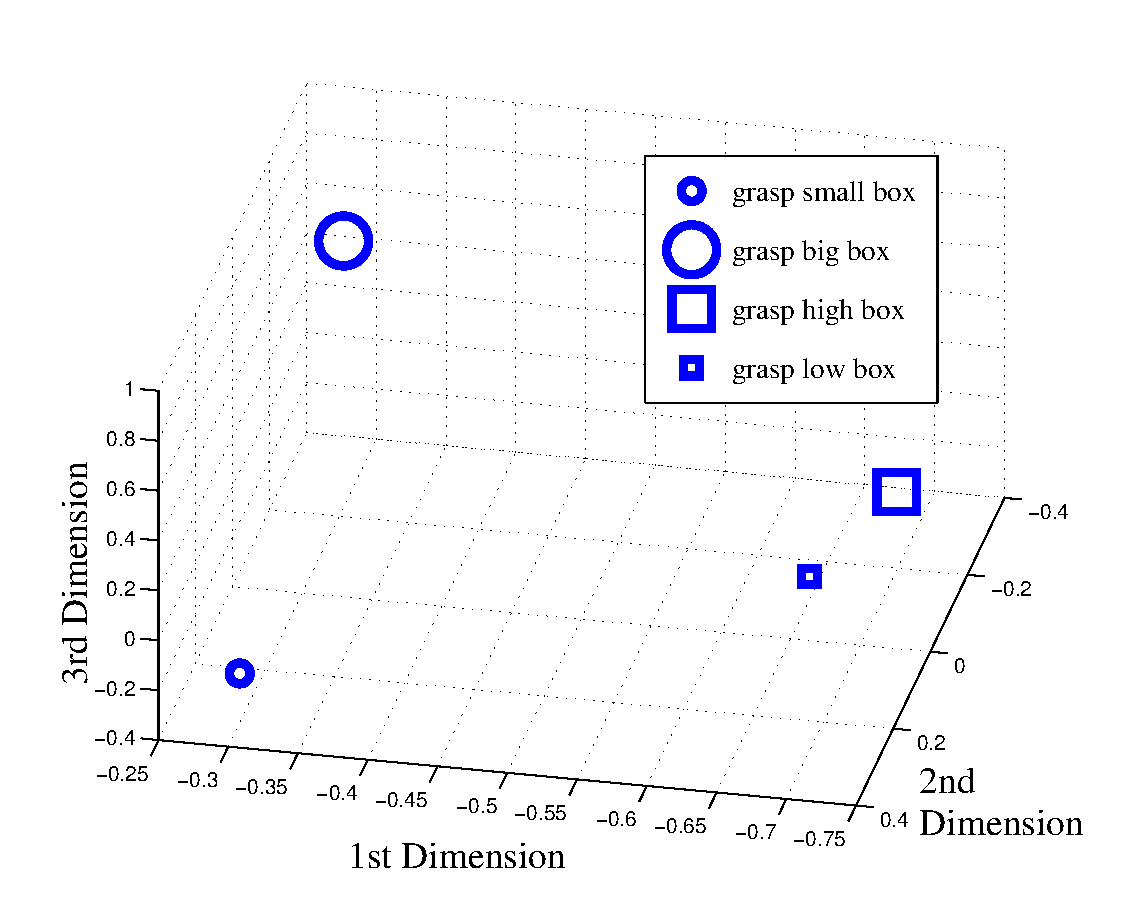
\includegraphics[width=12cm]{./fig_cha5/pss2.eps}
  \caption{ \scriptsize{Proto-symbol space constructed by four motion primitives}
}
    \label{fig:pss}
\end{figure}


\subsection{Grasping different sizes boxes}
\label{cha5:sec3:graspsize}
In this scenario we demonstrate the strategies of grasping different sizes of boxes. The boxes are placed on a cylindrical stand with 84$cm$ height. The human demonstrator stands 20$cm$ in front of the cylindrical stand (Figure~\ref{fig:graspdemo}).

\begin{figure}
  \centering
  \subfloat[\scriptsize{Motion 1}]{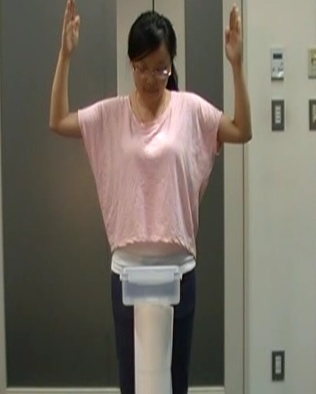
\includegraphics[width=4cm]{./fig_cha5/demosbox1s.jpg}}
  \subfloat[\scriptsize{Motion 2}]{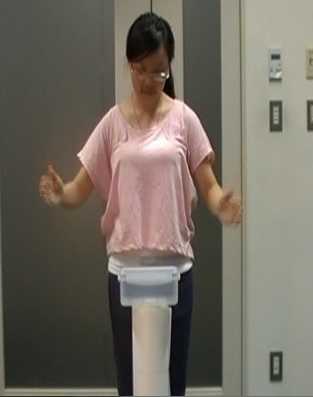
\includegraphics[width=3.96cm]{./fig_cha5/demosbox3s.jpg}}
  \subfloat[\scriptsize{Motion 3}]{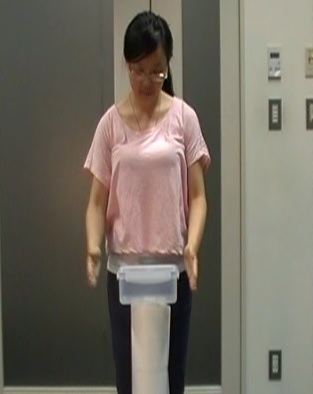
\includegraphics[width=4cm]{./fig_cha5/demosbox4s.jpg}}
  \subfloat[\scriptsize{Motion 4}]{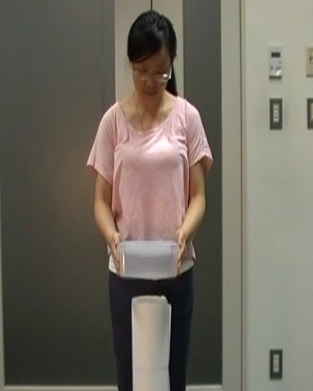
\includegraphics[width=4cm]{./fig_cha5/demosbox6s.jpg}}
  \hspace{1cm}
  \subfloat[\scriptsize{Motion 1}]{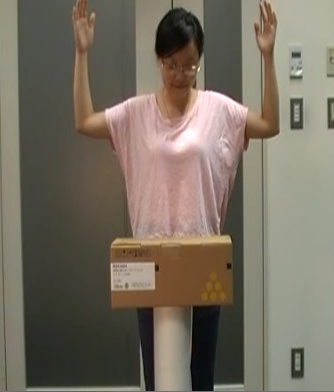
\includegraphics[width=4.2cm]{./fig_cha5/demopinkbox1s.jpg}}
  \subfloat[\scriptsize{Motion 2}]{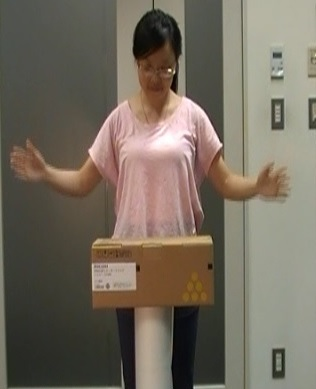
\includegraphics[width=4cm]{./fig_cha5/demopinkbox3s.jpg}}
  \subfloat[\scriptsize{Motion 3}]{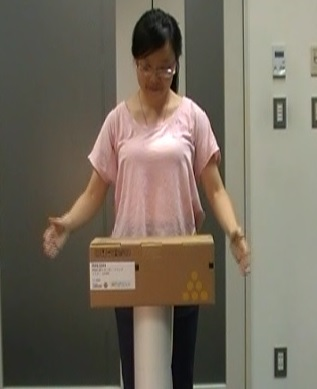
\includegraphics[width=4cm]{./fig_cha5/demopinkbox4s.jpg}}
  \subfloat[\scriptsize{Motion 4}]{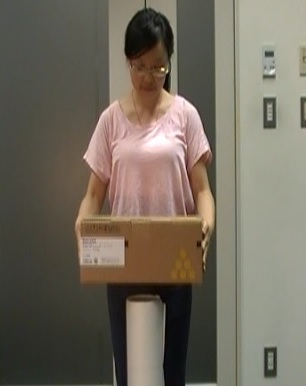
\includegraphics[width=3.9cm]{./fig_cha5/demopinkbox6s.jpg}}
  \caption{ \scriptsize{(a)-(d): Human demonstrating bi-manual grasp of a small box (size 20$cm$(length) $\times$ 15$cm$(width) $\times$ 10$cm$(height)). (e)-(h): Human demonstrating bi-manual grasp of a big box (size 40$cm$(length) $\times$ 20$cm$(width) $\times$ 15$cm$(height))}
}
  \label{fig:graspdemo}
\end{figure}

Figure~\ref{fig:graspdemo} shows the motion sequences. As can be seen from the figure, for grasping the small box, the hands move directly to it, while for grasping the big box, the arms first open to create a certain distance between hands and then close to reduce the distance until contact with the box. This is to avoid unwanted collision with the box during reaching.

New motions are then generated by mixing the demonstrations. To learn the effect of the motions, all demonstrated and generated motions are performed by the robot.
The sizes of the boxes are initially estimated by forward kinematics, and then verified by robot executing the motion to grasp a box. The motion that can hold a box and lift it vertically without any slipping is consider to be a successful grasp. Table~\ref{trainmixing} shows the mixing coefficients of the motions and the corresponding size of boxes of successful grasps. Note that mixing coefficients of them always sum to 1. When we make the mixing coefficient to be 1 for one motion and 0 for the other, the generated motion simply corresponds to the motion with mixing coefficient 1. Linear regression is the applied to find out the correlation between the mixing coefficients and the box sizes.


\begin{table}
\centering
\renewcommand{\arraystretch}{1.5}
    \begin{tabular}{|>{\centering\arraybackslash}p{8cm}|>{\centering\arraybackslash}p{4cm}|}
    \hline
    Mixing Coefficient of the Interpolation Points & Box size of successful grasps ($cm$)   \\ \hline
    0(small box) 1(big box)   & 43\\ \hline
    0.2(small box) 0.8(big box)   & 39\\ \hline
    0.5(small box) 0.5(big box)   & 35\\ \hline
    0.8(small box) 0.2(big box)   & 28\\ \hline
    1(small box) 0(big box)   & 25\\ \hline
    \end{tabular}
    \caption{ \scriptsize{Mixing coefficient of the interpolation points and the box Size of Successful grasps (training)}}

    \label{trainmixing}
\end{table}

\begin{figure}
  \centering
  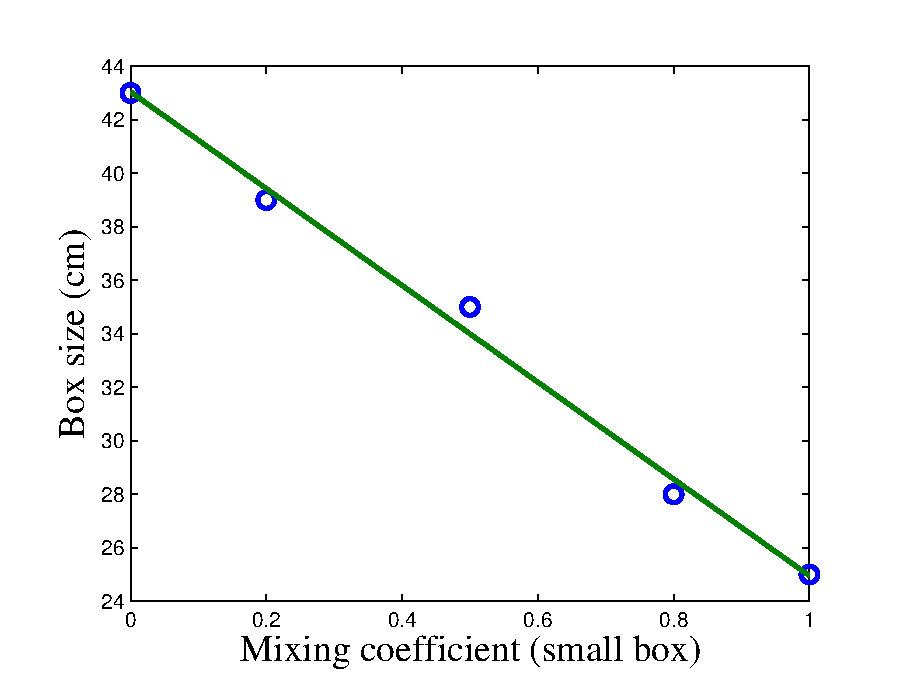
\includegraphics[width=12cm]{./fig_cha5/regression_size.eps}
  \caption{ \scriptsize{Linear regression of the interpolation points}
}
  \label{regression}
\end{figure}


\begin{table}
\centering
\renewcommand{\arraystretch}{1.5}
    \begin{tabular}{|>{\centering\arraybackslash}p{4cm}|>{\centering\arraybackslash}p{8cm}|}
    \hline
    Given Box Size & Predicted Mixing Coefficient \\ \hline
    27    &0.89(small box) 0.11(big box)\\ \hline
    30     &0.72(small box) 0.27(big box)\\ \hline
    36    &0.44(small box) 0.56(big box)\\ \hline
    40     &0.16(small box) 0.74(big box)\\ \hline
    \end{tabular}
    \caption{ \scriptsize{Given Box Sizes ($cm$) and the Predicted Mixing Coefficient (testing)}}
    \label{predictmixing}
\end{table}



Figure~\ref{regression} shows the linear regression result of the mixing coefficients and the size of successful grasped boxes. With the regression result, given a size of box, the mixing coefficient of generating a corresponding grasping motion can be deduced. To test this method, we apply this method to grasp four un-demonstrated boxes with different sizes. All of them can be successfully lifted by the synthesis grasping motions. Table~\ref{predictmixing} lists the given boxes size and the computed mixing coefficient and Figure~\ref{graspdemo2} shows the corresponding motions.


\begin{figure}
  \hspace{-2.2cm}
  \begin{minipage}[c]{1\textwidth}
  \subfloat[\scriptsize{Motion 1}]{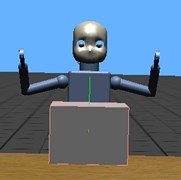
\includegraphics[width=4cm]{./fig_cha5/icub27box1_crop.jpg}}
  \subfloat[\scriptsize{Motion 2}]{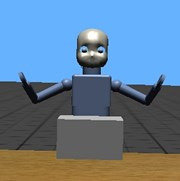
\includegraphics[width=3.96cm]{./fig_cha5/icub27box2_crop.jpg}}
  \subfloat[\scriptsize{Motion 3}]{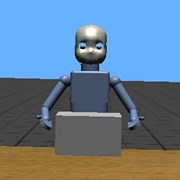
\includegraphics[width=4cm]{./fig_cha5/icub27box3_crop.jpg}}
  \subfloat[\scriptsize{Motion 4}]{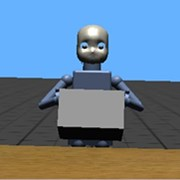
\includegraphics[width=4cm]{./fig_cha5/icub27box4_crop.jpg}}
  \end{minipage}

  \hspace{-2.2cm}
  \begin{minipage}[c]{1\textwidth}
  \subfloat[\scriptsize{Motion 1}]{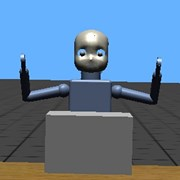
\includegraphics[width=4cm]{./fig_cha5/icub30box1_crop.jpg}}
  \subfloat[\scriptsize{Motion 2}]{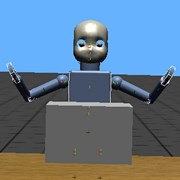
\includegraphics[width=4cm]{./fig_cha5/icub30box2_crop.jpg}}
  \subfloat[\scriptsize{Motion 3}]{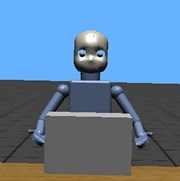
\includegraphics[width=4cm]{./fig_cha5/icub30box3_crop.jpg}}
  \subfloat[\scriptsize{Motion 4}]{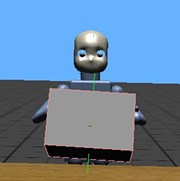
\includegraphics[width=4cm]{./fig_cha5/icub30box4_crop.jpg}}
  \end{minipage}

  \hspace{-2.2cm}
  \begin{minipage}[c]{1\textwidth}
  \subfloat[\scriptsize{Motion 1}]{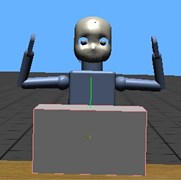
\includegraphics[width=4cm]{./fig_cha5/icub35box1_crop.jpg}}
  \subfloat[\scriptsize{Motion 2}]{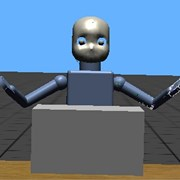
\includegraphics[width=4cm]{./fig_cha5/icub35box2_crop.jpg}}
  \subfloat[\scriptsize{Motion 3}]{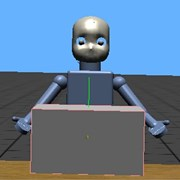
\includegraphics[width=4cm]{./fig_cha5/icub35box3_crop.jpg}}
  \subfloat[\scriptsize{Motion 4}]{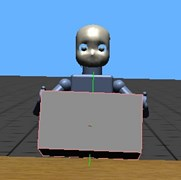
\includegraphics[width=4cm]{./fig_cha5/icub35box4_crop.jpg}}
  \end{minipage}

  \hspace{-2.2cm}
  \begin{minipage}[c]{1\textwidth}
  \subfloat[\scriptsize{Motion 1}]{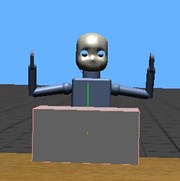
\includegraphics[width=4cm]{./fig_cha5/icub40box1_crop.jpg}}
  \subfloat[\scriptsize{Motion 2}]{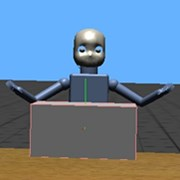
\includegraphics[width=4cm]{./fig_cha5/icub40box2_crop.jpg}}
  \subfloat[\scriptsize{Motion 3}]{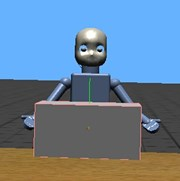
\includegraphics[width=4cm]{./fig_cha5/icub40box3_crop.jpg}}
  \subfloat[\scriptsize{Motion 4}]{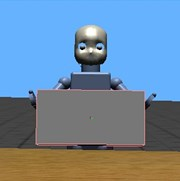
\includegraphics[width=4cm]{./fig_cha5/icub40box4_crop.jpg}}
  \end{minipage}

  \caption{ \scriptsize{Robot grasping different boxes with the generated motions.
  (a)-(d) Box size 0.27$cm$. (e)-(h) Box size 0.3$cm$. (i)-(l) Box size 0.35$cm$. (m)-(p) Box size 0.4$cm$.}
}
    \vspace{-0.5cm}
    \label{graspdemo2}
\end{figure}

\subsection{Grasping boxes from different positions}
\label{sbsec:diffheight}
In this scenario the goal is to grasp boxes from different heights. Two motions are demonstrated to grasp a high and a low box. In the demonstrations the high box is placed at the height of $150 cm$ and the low box is placed at $70 cm$. In this case, the two demonstrations are not only different in the arm trajectories but also different in the time duration (Figure~\ref{highlowjoint}). The motion of grasping the high box lasts shorter than grasping the low box as the initial hand position is closer to the box position. At the same time the lifting parts of the motions are different: for the high box the lifting distance is smaller than the low box because of the joint limits of the arms.

\begin{figure}
    \centering
    \subfloat[\scriptsize{Grasping box in a low position}]{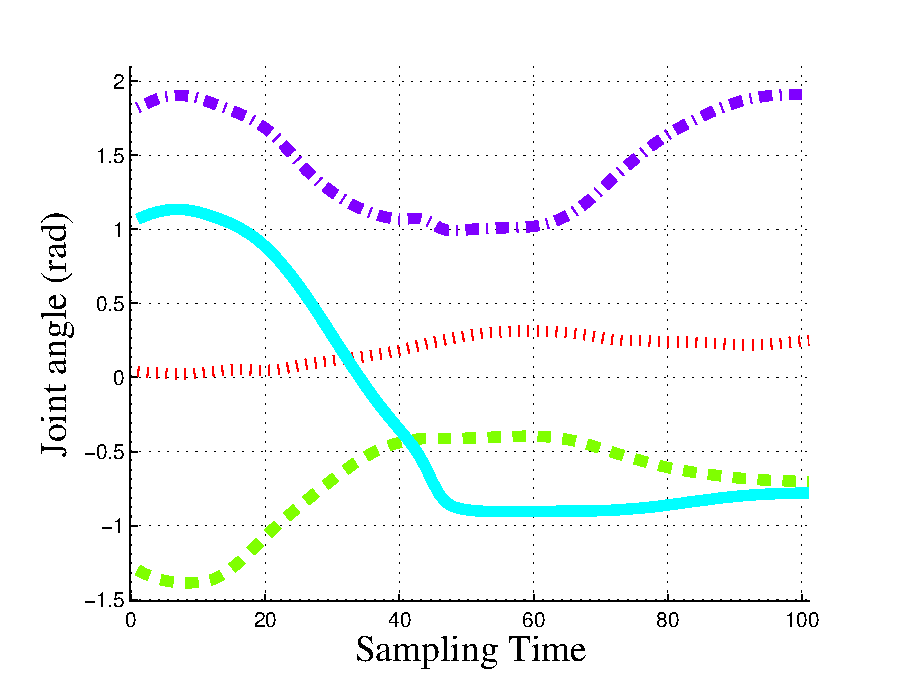
\includegraphics[width=8cm]{./fig_cha5/joint_sbox_adj.eps}}
    \subfloat[\scriptsize{Grasping box in a high position}]{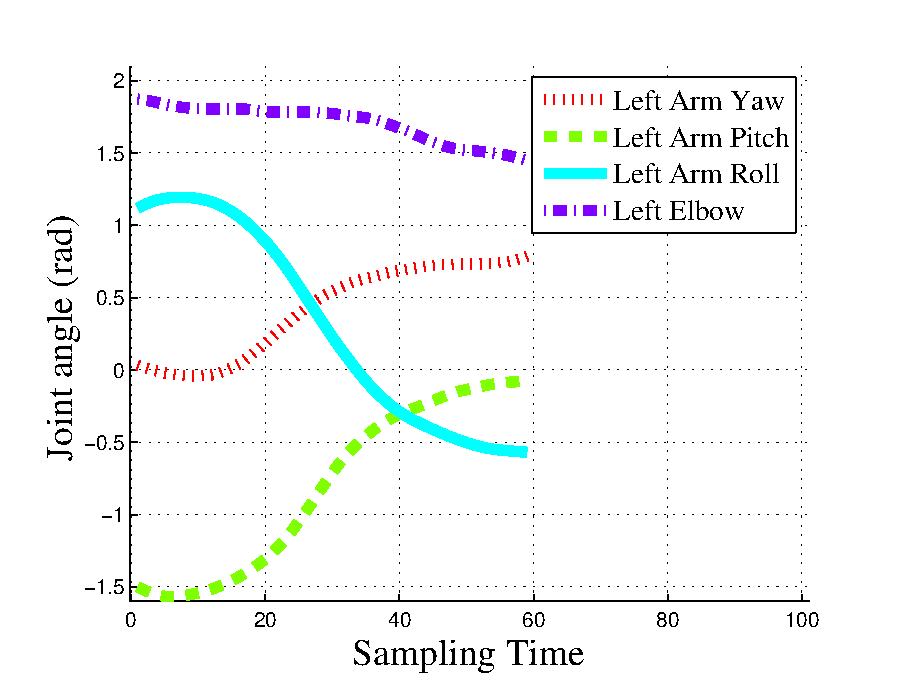
\includegraphics[width=8cm]{./fig_cha5/joint_ssbox_high356.eps}}
    \caption{ \scriptsize{(a) Left arm motion of a human demonstration of grasping a low box. (b) Left arm motion of a human demonstration of grasping a high box.}}
\label{highlowjoint}
\end{figure}
Following the same process as described above, we interpolate between the motions for grasping low box and high box (Table~\ref{trainhigh}). We apply linear regression and hence find out the correlation between the mixing coefficients and the heights of the box (Figure~\ref{highregression}).

With the learned correlation, we query the mixing coefficients for four different un-demonstrated heights (Table~\ref{predictmixing_high}). The generated motions are tested with the Webots iCub, which successfully lifted all the boxes. %Besides the height of the box, the time of performing the task and the lifting distances are also interpolated .

\begin{table}
\centering
\renewcommand{\arraystretch}{1.5}
    \begin{tabular}{|>{\centering\arraybackslash}p{8cm}|>{\centering\arraybackslash}p{4cm}|}
    \hline
    Mixing Coefficient &  Box height($cm$)  \\ \hline
    0(high box) 1(low box)   & 49\\ \hline
    0.2(high box) 0.8(low box)   & 53\\ \hline
    0.5(high box) 0.5(low box)   & 58\\ \hline
    0.8(high box) 0.2(low box)   & 62\\ \hline
    1(high box) 0(low box)   & 64\\ \hline
    \end{tabular}
    \caption{\scriptsize{Mixing coefficient of the interpolation points and the box heights (center of mass from the ground) of successful grasps (training).}}
    \vspace{-0.5cm}
    \label{trainhigh}
\end{table}

\begin{figure}
  \centering
  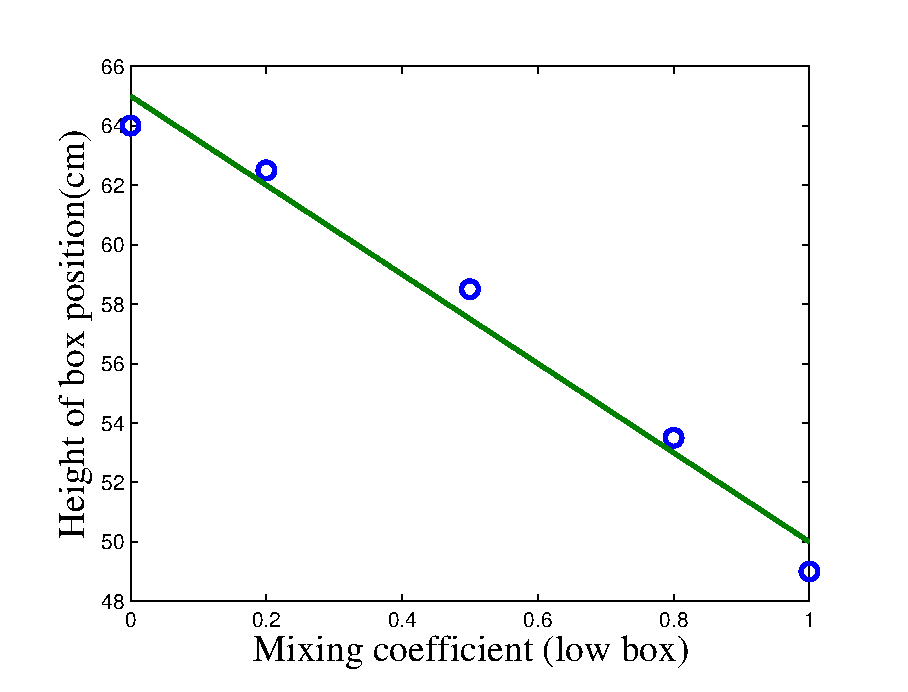
\includegraphics[width=12cm]{./fig_cha5/regression_high.eps}
  \caption{ \scriptsize{Linear regression of the interpolation points}
}
    \vspace{-0.5cm}
    \label{highregression}
\end{figure}

\begin{table}
\centering
\renewcommand{\arraystretch}{1.5}
    \begin{tabular}{|>{\centering\arraybackslash}p{4cm}|>{\centering\arraybackslash}p{8cm}|}
    \hline
    Given Box Height & Predicted Mixing Coefficient \\ \hline
    50    &0.02(high box) 0.98(low box)\\ \hline
    55     &0.34(high box) 0.66(low box)\\ \hline
    60    &0.66(high box) 0.34(low box)\\ \hline
    63     &0.86(high box) 0.14(low box)\\ \hline
    \end{tabular}
    \caption{\scriptsize{Given Box Height ($cm$) and the Predicted Mixing Coefficient (testing)}}
    \label{predictmixing_high}
\end{table}

\begin{figure*}
  \centering
  \hspace{-2.2cm}
  \begin{minipage}[c]{1\textwidth}
  \subfloat[\scriptsize{Motion 1}]{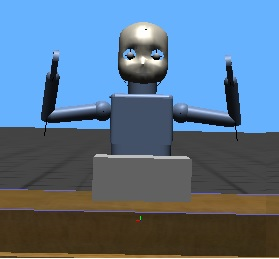
\includegraphics[width=4cm]{./fig_cha5/sbox_high356_ssbox_adj_005_095_1.jpg}}
  \subfloat[\scriptsize{Motion 2}]{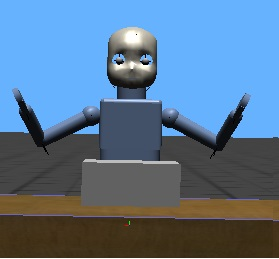
\includegraphics[width=4cm]{./fig_cha5/sbox_high356_ssbox_adj_005_095_2.jpg}}
  \subfloat[\scriptsize{Motion 3}]{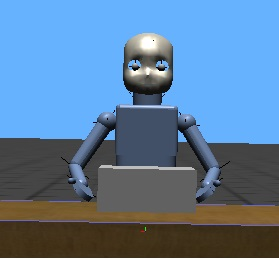
\includegraphics[width=4cm]{./fig_cha5/sbox_high356_ssbox_adj_005_095_3.jpg}}
  \subfloat[\scriptsize{Motion 4}]{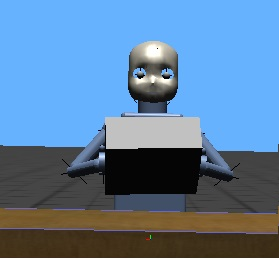
\includegraphics[width=4cm]{./fig_cha5/sbox_high356_ssbox_adj_005_095_4.jpg}}
  \end{minipage}

  \hspace{-2.2cm}
  \begin{minipage}[c]{1\textwidth}
  \subfloat[\scriptsize{Motion 1}]{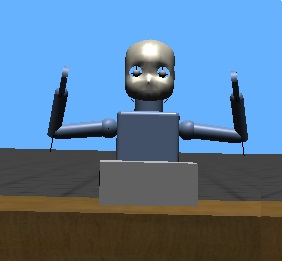
\includegraphics[width=4cm]{./fig_cha5/sbox_high356_ssbox_adj_167_833_1.jpg}}
  \subfloat[\scriptsize{Motion 2}]{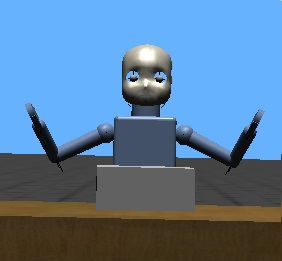
\includegraphics[width=4cm]{./fig_cha5/sbox_high356_ssbox_adj_167_833_2.jpg}}
  \subfloat[\scriptsize{Motion 3}]{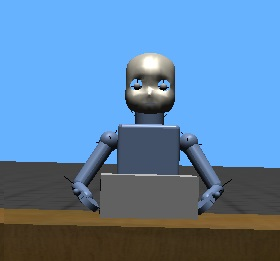
\includegraphics[width=4cm]{./fig_cha5/sbox_high356_ssbox_adj_167_833_3.jpg}}
  \subfloat[\scriptsize{Motion 4}]{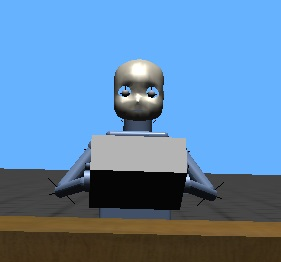
\includegraphics[width=4cm]{./fig_cha5/sbox_high356_ssbox_adj_167_833_4.jpg}}
  \end{minipage}

  \hspace{-2.2cm}
  \begin{minipage}[c]{1\textwidth}
  \subfloat[\scriptsize{Motion 1}]{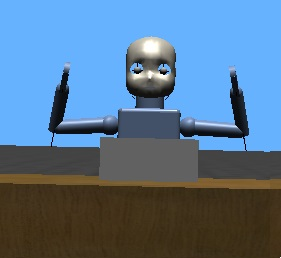
\includegraphics[width=4cm]{./fig_cha5/sbox_high356_ssbox_adj_433_567_1.jpg}}
  \subfloat[\scriptsize{Motion 2}]{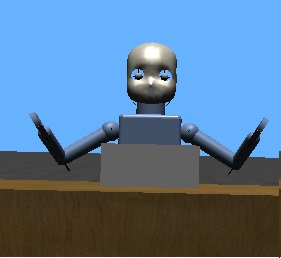
\includegraphics[width=4cm]{./fig_cha5/sbox_high356_ssbox_adj_433_567_2.jpg}}
  \subfloat[\scriptsize{Motion 3}]{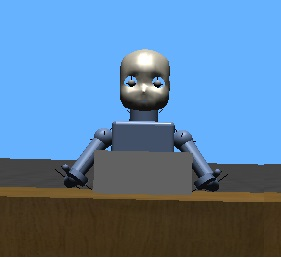
\includegraphics[width=4cm]{./fig_cha5/sbox_high356_ssbox_adj_433_567_3.jpg}}
  \subfloat[\scriptsize{Motion 4}]{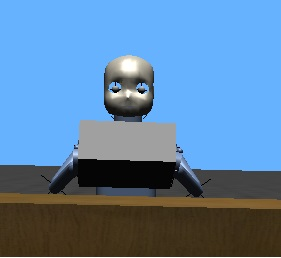
\includegraphics[width=4cm]{./fig_cha5/sbox_high356_ssbox_adj_433_567_4.jpg}}
  \end{minipage}

  \hspace{-2.2cm}
  \begin{minipage}[c]{1\textwidth}
  \subfloat[\scriptsize{Motion 1}]{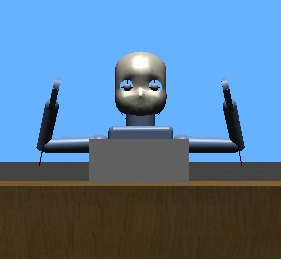
\includegraphics[width=4cm]{./fig_cha5/sbox_high356_ssbox_adj_667_333_1.jpg}}
  \subfloat[\scriptsize{Motion 2}]{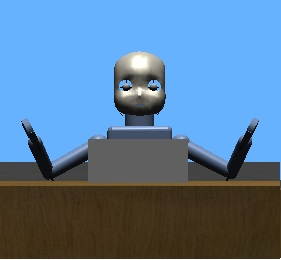
\includegraphics[width=4cm]{./fig_cha5/sbox_high356_ssbox_adj_667_333_2.jpg}}
  \subfloat[\scriptsize{Motion 3}]{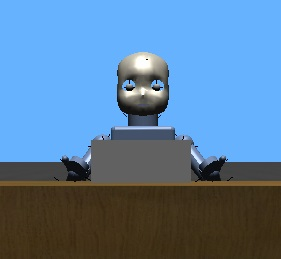
\includegraphics[width=4.02cm]{./fig_cha5/sbox_high356_ssbox_adj_667_333_3.jpg}}
  \subfloat[\scriptsize{Motion 4}]{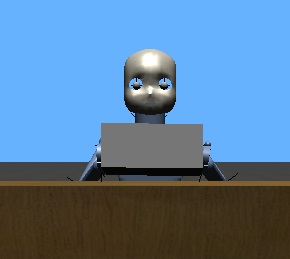
\includegraphics[width=4.1cm]{./fig_cha5/sbox_high356_ssbox_adj_667_333_4.jpg}}
  \end{minipage}

  \caption{ \scriptsize{Robot grasping boxes from different heights with the generated motions.
  (a)-(d) Box at height 50$cm$. (e)-(h) Box at height 55$cm$. (i)-(l) Box at height 60$cm$. (m)-(p) Box at height 63$cm$.}
}
    \label{graspdemo2}
\end{figure*} 
\section{Discussion}
\label{cha5:sec4}

The system we present in this chapter uses the mimesis model to learn motion primitives for object manipulation. It provides an easy to use interface for robot motion generation. Motion primitives are the elementary motions that accomplish basic functions. Recent brain research~\cite{bizzi2008combining} provide more evidences to support the hypothesis that, in order to reduce the degree of freedom, the vertebrate motor system generate motions by combining a small number of motor primitives. Our experiment shows that by combining two motion primitives (8 d.o.f) indeed we can generate many different motion patterns. This framework largely simplifies the modeling of motion primitives.

From the function point of view, the motion primitives form the vocabulary of motions. This naturally allows us to label motion primitives by words. In our system, each motion primitive is symbolized in the proto-symbol space and labeled by its effects, i.e. ``grasp high box", ``grasp low box" and etc. This provides a linguistic interface for the human to instruct robot motion, by giving language instructions like ``go lower to grasp the box". By matching the words in human instruction and the labels of the motion primitives, the robot will be able to adjust the mixing coefficient and generate new motion to execute the command.

We implement the system in the Webots simulator with the iCub robot. The interpolation of the proto-symbols produces new motion primitives. The correlation between the new motions and their effects are learnt using first order linear regression. In our future work of learning more complex motion primitives, higher order or nonlinear regression may need to be employed.

The presented experiment provides a good starting point for our future study in learning more motion primitives for object manipulation. It shows that it is possible to directly control the outcome of the motion pattern, without fine tuning different variables in the model. This has the advantage, from the user point of view, of planning the motion primitives more intuitively. In this chapter, we show that with the mimesis model control in one dimension (object size, object height) works effectively. In the future work, we will further study the control in multi-dimension, i.e. interpolation between multi-proto-symbols.



